\chapter{Synthetic Aperture Radar Basics}\label{chp:background}%\Cref{sec:pr_obs}
% 

%------------------------------------
%	
%------------------------------------




This chapter presents some basics of remote sensing that we will use in the rest of the document and focuses on the theory of SAR.


\section{Remote Sensing} \label{sec:pr_obs}

Remote sensing is the practice of deriving information about the Earth's land using images acquired from elevated platforms like airplanes or satellites in space, using electromagnetic radiation across various regions of the electromagnetic spectrum~\citep{campbell2011introduction}.

The word “radar” was originally an acronym, RADAR, for “radio detection and ranging”.
Today, the technology is so common that the word has become a standard English noun.
The history of radar extends to the early days of modern electromagnetic theory. 
In 1886, Hertz demonstrated reflection of radio waves, and in 1900 Tesla described a concept for electromagnetic detection and velocity measurement in an interview.
Early radar development was driven by military necessity, and the military is still a major user and developer of radar technology.
Radar is also an essential sensor for emerging autonomous driving systems. 
Finally, spaceborne and airborne radar is an important tool in mapping earth topology and environmental characteristics such as water and ice conditions, forestry conditions, land usage, and pollution~\citep{richards2005fundamentals}.

In 1951 Carl Wiley developed synthetic aperture radar while working at the Goodyear Aircraft Company. 
Using a technique known as Doppler beam sharpening, the signals from a series of locations are summed to produce a finer azimuth resolution than 
the antenna beamwidth can achieve~\citep{wiley1985synthetic}. 
Since then, the technology has found a multitude of applications in the scientific, military, and civilian communities alike. Due to the numerous uses, SAR technology has been a topic of constant
research and development.

\subsection{Remote Sensors}
Remote sensors collect data remotely by measuring electromagnetic (EM) radiation within specific spectral ranges,  often called bands. 
When they are deployed on satellites or mounted on aircraft, they are called spaceborne and airborne remote sensors, respectively.
 Spaceborne remote sensors orbit the Earth at heights of 500 to 800 km~\citep{everaerts2005pegasus}, providing data in a wide range of ground resolutions, and at various polarizations and radar bands. 

There are two types of remote sensors acquiring information in fundamentally different ways.
Optical sensors are passive imaging devices, which means they take advantage of existing sources of illumination and the natural reflective properties of objects to form
images. 
In the case of optical Earth observation imagery, the sun is used as a global illumination source. 
Thus, optical image sensors tend to operate on a sun-synchronous orbit to ensure the scene is well illuminated during acquisition. 
On the other hand, SAR uses the principle of active sensing, whereby the sensor acts as both an illumination source as well as the acquisition unit. 
A scene is thus imaged by alternating between emitting bursts of EM-radiation and measuring the strength and time delay of the reflected signal. 
The proportion of the signal which is reflected towards the sensor by an object is known as \textit{backscatter}.
\subsection{The Electromagnetic Spectrum}
Given that objects interact (reflect and absorb) different parts of the EM-spectrum in a unique manner, several realizations of optical and SAR sensors exist, each designed for
a specific purpose and to take advantage of the properties observable within a particular part of the EM-spectrum.
Optical sensors detect very high-frequency radiation within the visible to thermal infrared section of the EM-spectrum.
In contrast, SAR sensors operate at much lower frequencies within the microwave section of the spectrum.
It is this use of lower frequencies which allow SAR sensors to be mostly independent of atmospheric conditions.
The same, however, is not true for optical sensors which require clear atmospheric conditions to observe ground level reflections within the visible light and near-infrared spectrum.

In general, optical sensors can be classified by the number of spectral bands they image into hyperspectral, multispectral, and panchromatic sensors. 
Hyperspectral sensors image the full optical subsection of the EM spectrum into hundreds of narrow spectral bands, while panchromatic sensors image the visible light spectrum using a single, wide spectral band~\citep{Sara2021}.
Similarly, SAR sensors can also be classified based on their operational bandwidth into C, L and X-band, with L-band being the lowest frequency and thus the highest level of vegetation and soil penetration.
However, due to the relationship between wave-length and spatial resolution present in SAR imagery~\citep{cumming2005digital}, X-band imagery exhibits the highest spatial resolution and thus provides the detailed information about surface structure. 
In optical imagery, a similar trade-off exists, except it is between spatial resolution and spectral resolution. 
Due to data storage and throughput constraints hyperspectral and multispectral images tend to have a lower resolution than panchromatic imagery.

The operational frequency and bandwidth of each of these sensors within the EM-spectrum is further described by Figure~\ref{fig:EM-spectrum}.
%%% The source is in ../../Images/PNG/EM-spectrum.PNG
	\begin{figure}[H]
    \centering
    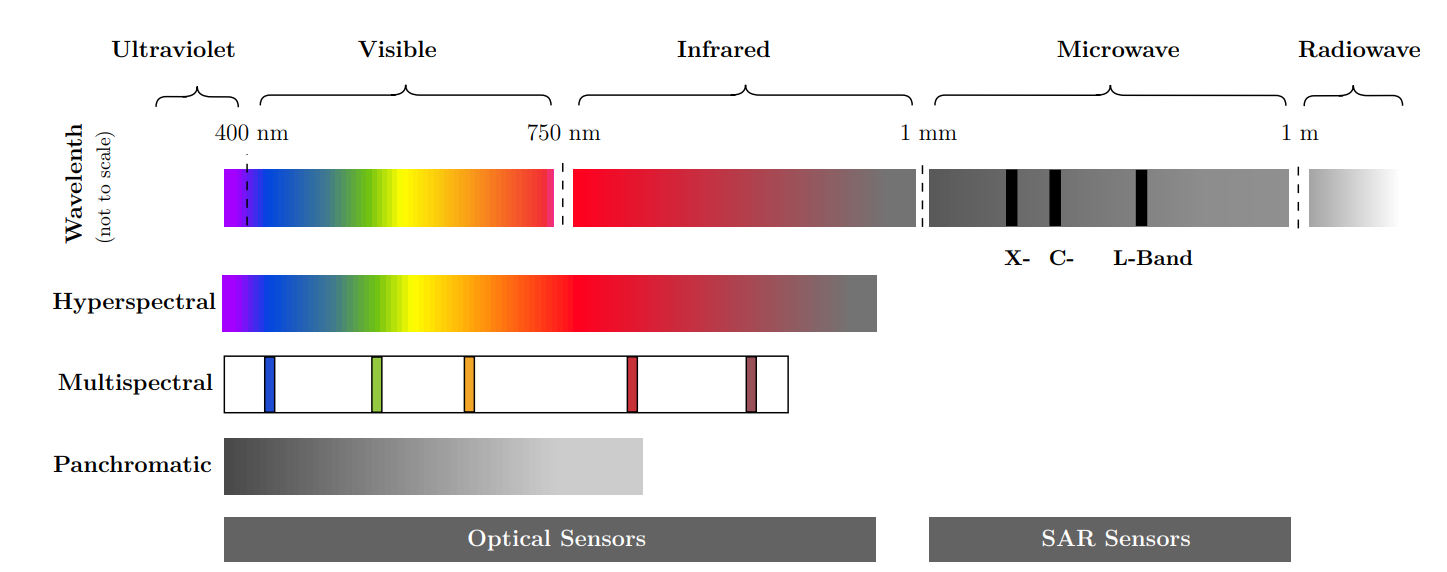
\includegraphics[width=0.9\textwidth]{../../Images/PNG/sensor.png}
    %\decoRule
    \caption[Spectral regions of sensors within the electromagnetic spectrum.]{Spectral regions of optical sensors and radar sensors within the electromagnetic spectrum,~\citep{zhang2022synthetic}.}
    \label{fig:EM-spectrum}
\end{figure}
SAR sensors provide radar images of the Earth’s surface, which are chosen in this work.
Table~\ref{tab:bands} contains the band with the associated frequency and wavelength. 
The wavelength range is very important, since it determines the interaction between radar signals and surfaces, as well as the penetration depth of the microwave
signals.

\setlength{\tabcolsep}{6.0pt}
\begin{table}[!htb]
\caption[Different bands in microwave remote sensing]{\label{tab:bands}Different bands in microwave remote sensing,~\citep{Moreira2013}.}
\centering
\begin{tabular}[t]{cccccc}
\toprule
 \textbf{Band} & \multicolumn{1}{c}{\textbf{Frequency} $\left[\text{GHz}\right]$} & \multicolumn{1}{c}{\textbf{Wavelength} $\left[\text{cm}\right]$} \\
\midrule
Ka & $\,25.0$--$40.0$ & $\phantom{-}0.75$--$1.2$ \\
Ku & $\,12.0$--$17.6$ & $\phantom{-}\,1.7$--$2.5$ \\
X  & $\phantom{-}7.5$--$12.0$  & $\phantom{-}2.5$--$4.0$   \\
C  & $ 3.7$--$7.5$ & $\phantom{-}4.0$--$8.0$   \\
S  & $2.0$--$3.7$   & $\phantom{-}\,8.0$--$15$    \\
L  & $1.0$--$2.0$   & $\phantom{-}15$--$30$   \\
P  & $0.3$--$1.0$ & $\phantom{-}\,30$--$100$  \\
\bottomrule
\end{tabular}
\end{table}

%\begin{longtable}{@{}
			%c
			%S[table-format=-4.1]@{--}S[table-format=2.5]
			%S[table-format=-2.1,
		%table-align-text-pre=false]@{--}S[table-format=2.6, table-align-text-pre=false]
			%%S[table-format=-2.1]@{--}S[table-format=2.3]
			%@{}}
		%%\caption{Las entradas de esta tabla están centradas correctamente, pero las distancias son difíciles de ajustar.}%
		%\caption[Different bands in microwave remote sensing]{\label{tab:bands}Different bands in microwave remote sensing,~\citep{Moreira2013}.}
		%\\
		%\toprule
		%\text{Band}            &
		%\multicolumn{2}{c}{\text{\textbf{Frequency} $\left[\text{GHz}\right]$}}        &
		%\multicolumn{2}{c}{\textbf{Wavelength} $\left[\text{cm}\right]$}          \\
		%\midrule
		%\endfirsthead
		%\midrule
		%\text{Band}            &
		%\multicolumn{2}{c}{\text{\textbf{Frequency} $\left[\text{GHz}\right]$}}        &
		%\multicolumn{2}{c}{\textbf{Wavelength} $\left[\text{cm}\right]$}          \\
		%\midrule
		%\endhead
		%Ka & 25.0 & 40.0 & 0.7 & 1.2 \\
		%Ku & 12.0 & 17.6 & 1.7 & 2.5 \\
		%X  & 7.5 & 12.0 & 2.5 & 4.0 \\
		%C  & 3.7 &7.5 & 4.0 & 8.0 \\
		%S  & 2.0 & 3.7 & 8.0 & 15 \\
		%L  & 1.0 & 2.0 & 15.0 & 30 \\
		%P  & 0.3 & 1.0 & 30.0 & 100 \\
		%\bottomrule
	%\end{longtable}
	
	

Table~\ref{tab:spacebornes} gives some examples of commonly used spaceborne SAR sensors, currently in operation. 
These include Radarsat-2 from the Canadian Space Agency (CSA), TerraSAR-X from the German Aerospace Center (DLR), ALOS PALSAR-2 from the Japan Aerospace Exploration Agency (JAXA), and Sentinel-1A/1B from the European Space Agency (ESA) (see Figure~\ref{fig:Sentinel-1n}), as well as Gaofen-3 from the China National Space Administration (CNSA).
\begin{figure}[H]
    \centering
    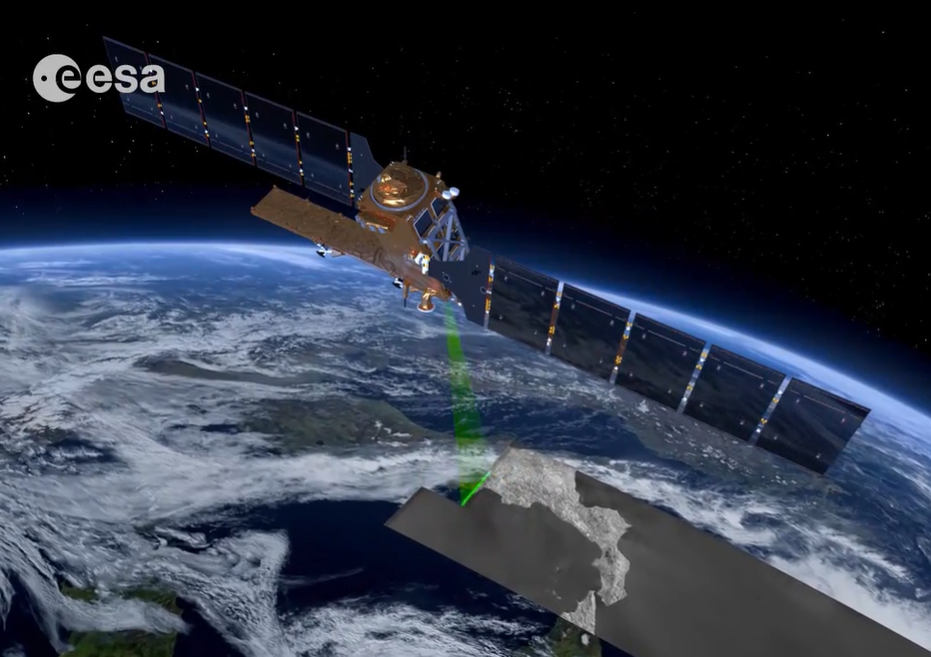
\includegraphics[width=0.6\textwidth]{../../Images/PNG/ESA_radar.png}
    %\decoRule
    \caption[Sentinel-1 radar.]{Sentinel-1 radar, (source \href{https://www.esa.int/Applications/Observing_the_Earth/Copernicus/Sentinel-1/Changing_lands}{ESA}).}
    \label{fig:Sentinel-1n}
\end{figure}


\setlength{\tabcolsep}{3.0pt}
\begin{table}[!htb]
\caption[List of operational typical spaceborne SAR systems]{\label{tab:spacebornes}List of operational typical spaceborne SAR systems.}
\centering
\setlength{\extrarowheight}{3.0pt} % 
\begin{tabular}[t]{lclccccc}
\toprule
\textbf{Mission/SAR} & \textbf{Agency} & \textbf{Launch} & \textbf{Band} & \textbf{Resolution} $\left[\text{m}\right]$ & \textbf{Coverage} $\left[\text{km}\right]$ & \textbf{Revisit} $\left[\text{days}\right]$ \\
\midrule
Radarsat-2 & CSA & 2007 & C & 9--100 & 18--500 & 24 \\
TerraSAR-X & DLR & 2007 & X & 0.25--40 & 10--150 & 11 \\
ALOS PALSAR-2 & JAXA & 2014 & L & 1--100 & 25--490 & 14 \\
Sentinel 1A/1B & ESA & 2014/2016 & C & 5--100 & 80--400 & 12 \\
Gaofen-3 & CNSA & 2016 & C & 1--500 & 10--650 & 29 \\
\bottomrule
\end{tabular}
\end{table}

\subsection{Scattering Mechanisms}
A SAR sensor measures the electromagnetic energy that is backscattered from the targets. 
There are lots of factors that can affect the radar backscatter, and they can be divided into two categories.

The first category relates to the SAR parameters, such as the frequency, polarization, and incident angle. If the frequency and
polarization parameters are fixed, the increasing incident angle causes the decreasing backscatter intensity from a homogeneous surface. 
Therefore, the intensity decreases gradually on SAR images from near range to far range. This effect must be taken into consideration during SAR image
interpretation.

The second category relates to the surface parameters, such as the surface roughness, the surface geometry, and the dielectric constant of the
surface. There are three basic groups of scattering mechanisms that can contribute to the returned signal: surface scattering, volume scattering, and hard target scattering.

\subsection{Electromagnetic Polarization}
An electromagnetic wave consists of a magnetic and an electric field.
These two fields are perpendicular to each other and also to the direction of wave propagation.

Apart from frequency, amplitude, and phase, an electromagnetic wave also contains polarization information.
Polarization is defined as the orientation of the oscillating electric field, which can be described in terms of two orthogonal basis vectors.
Electromagnetic waves are generally elliptically polarized, with linear or circular polarization as special cases.

Most of the SAR sensors use linear polarization on both the transmitter and the receiver. 
There are four linear polarization configurations in total:
\begin{itemize}
	\item HH (co-polarization): horizontal transmission and horizontal reception.
	\item HV (cross-polarization): horizontal transmission and vertical reception.
	\item VH (cross-polarization): vertical transmission and horizontal reception.
	\item VV (co-polarization): vertical transmission and vertical reception.
\end{itemize}
Historical SAR satellites carried single-polarized sensors, which support only one linear polarization. More recent sensors provide either dual-polarization
or quad-polarization capabilities. 
For quad-polarization SAR systems, they can transmit H- and V-polarized waveforms and receive both H and V simultaneously.

%An example of polarization is shown in Figure~\ref{}, where three intensity-format C-Band images of a region in Flevoland are observed, with VV and HV polarizations composited into an RGB image.
%An example of polarizations is shown in Figure~\ref{fig:pol}, from Sentinel-1 radar images in C-Band and intensity format of a region in Flevoland.
 Figure~\ref{fig:pol} \ref{fig:1a}--\ref{fig:2a} shows VH and VV polarization from Sentinel-1 radar images in C-Band of a region of Flevoland.
\begin{figure}[H]
  \centering
  \begin{subfigure}[b]{0.45\textwidth}
    \centering
    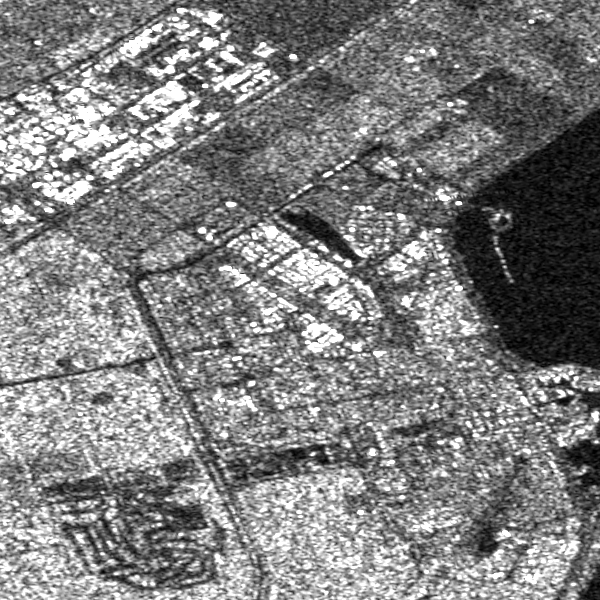
\includegraphics[width=.8\textwidth]{../../Images/PNG/Amplitude_VH.png}
    \caption{Cross-polarization (VH)}
    \label{fig:1a}
  \end{subfigure}
  \hfill
  \begin{subfigure}[b]{0.45\textwidth}
    \centering
    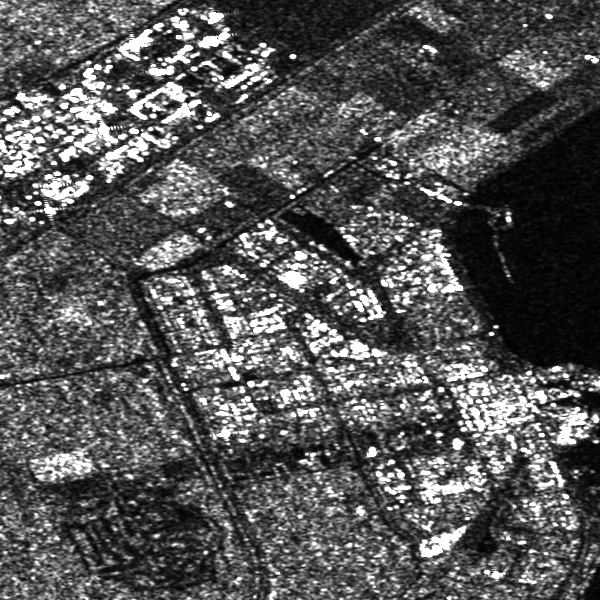
\includegraphics[width=.8\textwidth]{../../Images/PNG/Intensity_VV.png}
    \caption{Co-polarization (VV) }
    \label{fig:2a}
  \end{subfigure}
  %\hfill
  %\begin{subfigure}[b]{0.3\textwidth}
    %\centering
    %\includegraphics[width=\textwidth]{example-image-c}
    %\caption{}
    %\label{fig: Third figure}
  %\end{subfigure}
  \caption{Polarization in radar systems}
  \label{fig:pol}
\end{figure}




\section{SAR Image Acquisition}
SAR sensors utilize a single antenna to emit EM-signals and measure the corresponding magnitude, range and Doppler-shift of these signals in the
backscatter. 
As only a single detector element exists, SAR is based around the concept of synthesizing an aperture in the azimuth direction in order to form a 2-dimensional
image~\citep{Orth2018}. The angle between the SAR antenna and an object on the ground is known as the incidence angle, $\theta$, and it plays a large role in the geometric distortions which are
present in SAR imagery. Due to this imaging concept, the SAR image is formed along the slant range, where each pixel represents the accumulation of backscatter from points which are the same distance away from the sensor~\citep{cumming2005digital}. The acquisition geometry of  SAR sensors is depicted in Figure~\ref{fig:Sentinel-1}.

\begin{figure}[H]
    \centering
    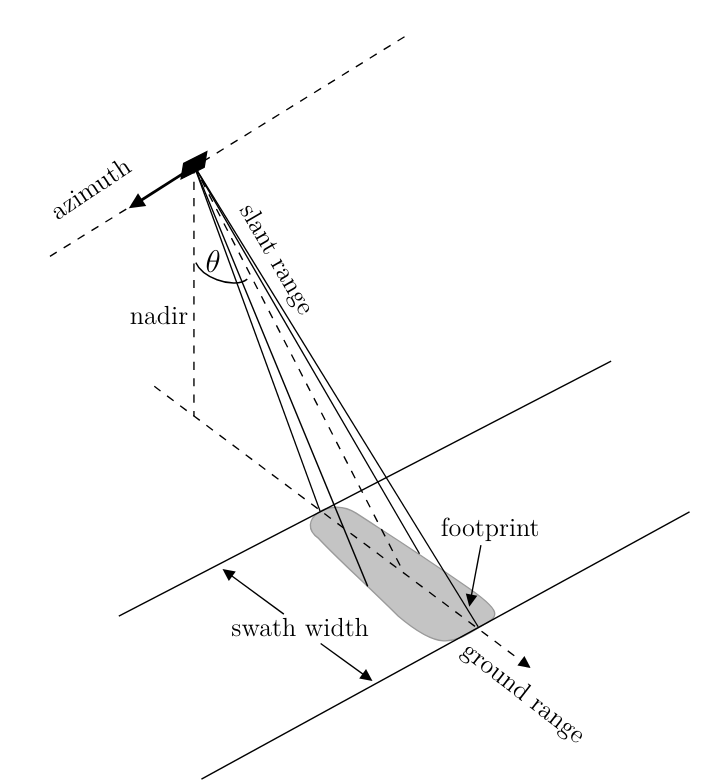
\includegraphics[width=0.5\textwidth]{../../Images/PNG/image_adquisition.png}
    %\decoRule
    \caption[Sentinel-1 radar.]{SAR image acquisition geometry,~\citep{hughes2020deep}.}
    \label{fig:Sentinel-1}
\end{figure}

\subsection{SAR resolution}
The resolution of the SAR image is one of the most important characteristics of the SAR system. 
SAR data pixels are characterized by spatial and temporal resolutions. Spatial resolution is defined as the ability of the SAR system to distinguish between two closely targets.
In SAR systems, there are two resolutions, azimuth resolution, and range resolution. 
Another resolution that should be taken into account when applying a multi-temporal time series analysis of the SAR data is the temporal resolution. 
It is determined by the revisit time of the SAR sensor at the same imaged area.


\subsection{Speckle Noise}
 
The interference of waves reflected during the acquisition process of SAR  images give rise to a multiplicative and non-Gaussian noise that characterizes them
and is known as speckle noise~\citep{oliver2004understanding}.
Since many elemental scatterers are located in one resolution cell, the final scattering response from the resolution cell is the coherent sum of thousands of individual scattering events.
The mutual interference results in a certain fluctuation in the amplitude and phase of the synthesized EM wave vectors, which make the “salt-and-pepper” noise  appear. 
%In the actual SAR images, speckle noise exists in the form of a multiplicative noise, which is manifested in the image as a drastic change in the image intensity.

%The interpretation of the SAR image is challenging due to the geometrical properties of the SAR imaging system and
%to the presence of speckle. Indeed, speckle is a multiplicative noise produced by interference among the backscatterings of
%the objects inside a resolution cell of the sensor~\citep{Argenti2013}.

The statistical distribution of the speckle is well known under certain conditions. Three main cases can be considered:
homogeneous, heterogeneous, and extremely heterogeneous areas. Homogeneous areas (such as fields, pasture, water bodies, etc)
are characterized by the lack of dominant scatterers, and the surface  can be considered stationary. This is the case of the
\textit{fully developed hypothesis for the speckle}~\citep{Frery1997}.

In Figure~\ref{fig:speckle}, SAR images depict speckle, a characteristic of SAR data due to its coherent imaging process. 
The images distinguish between fully developed speckle in homogeneous regions (Figure~\ref{fig:speckle} \ref{fig:s1}) and heterogeneous clutter in regions such as urban areas (Figure~\ref{fig:speckle} \ref{fig:s2}).
\begin{figure}[H]
  \centering
  \begin{subfigure}[b]{0.48\textwidth}
    \centering
    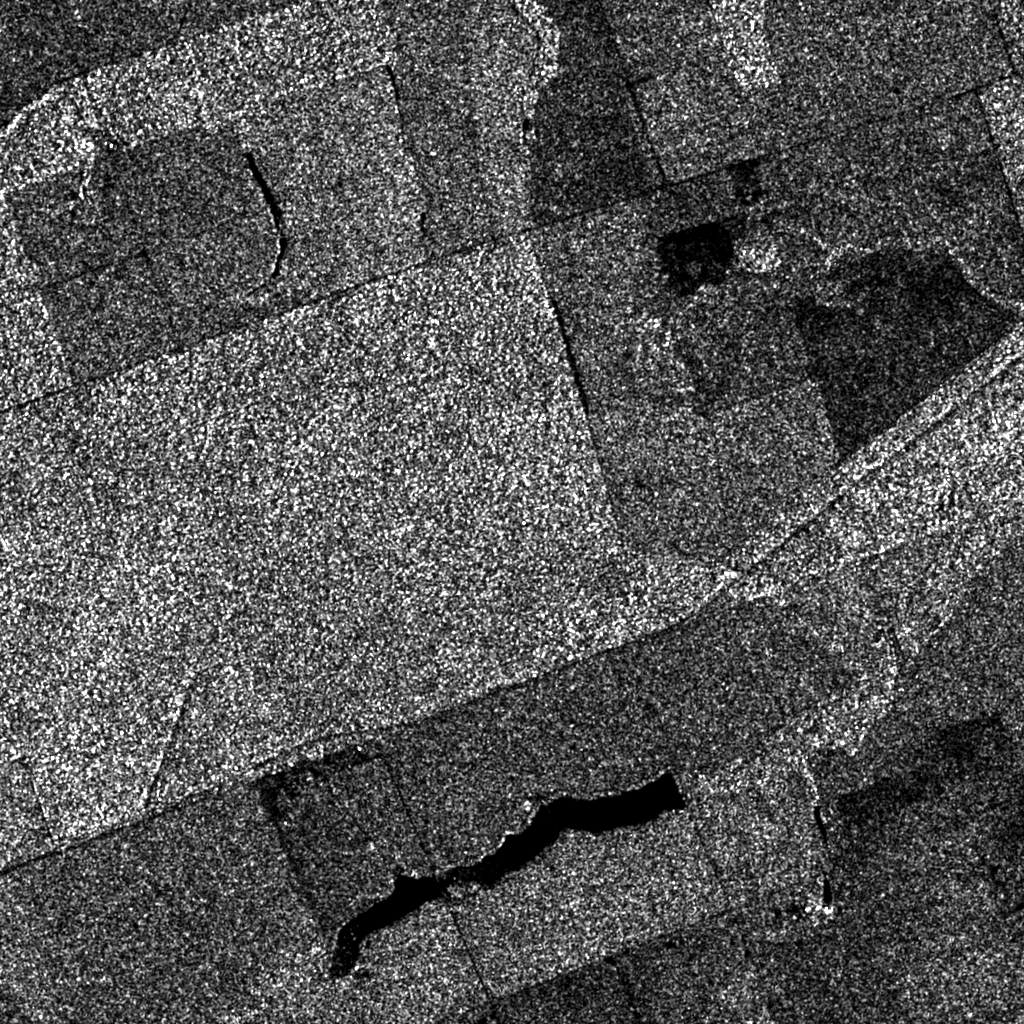
\includegraphics[width=.8\textwidth]{../../Images/PNG/Intensity_MG.png}
    \caption{Fully developed speckle (Homogeneous areas)}
    \label{fig:s1}
  \end{subfigure}
  \hfill
  \begin{subfigure}[b]{0.45\textwidth}
    \centering
    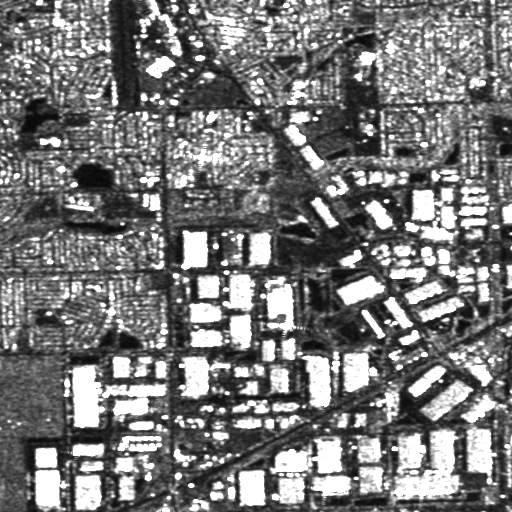
\includegraphics[width=.85\textwidth]{../../Images/PNG/urban_intensity.png}
    \caption{Heterogeneous clutter }
    \label{fig:s2}
  \end{subfigure}
  \caption{SAR image with speckle noise}
  \label{fig:speckle}
\end{figure}

\section{Dataset}
\subsection{Sentinel-1 SAR data processing}
The Sentinel-1 images were obtained from the Alaska Satellite Facility (ASF) at \url{https://search.asf.alaska.edu/#/} and by the European Space Agency via Copernicus Data Space Ecosystem at \url{https://dataspace.copernicus.eu/} (see Figure~\ref{fig:alaska-area1}).

The SAR images downloaded were pre-processed using the Sentinel Application Platform (SNAP) Toolbox developed by ESA (see Figure~\ref{fig:alaska-areaf}). 

%The following images describe the preprocessing steps applied to the SAR data: 
The following steps were applied to the SAR data during pre-processing:

\begin{enumerate}
    \item Importing the SAR image into SNAP.
    \item Creating a subset to focus on the area of interest.
    \item Performing Geometric Correction, which includes Range Doppler Terrain Correction.
    \item Exporting the processed data in ENVI format for further analysis.
\end{enumerate}



\begin{figure}[H]
    \centering
    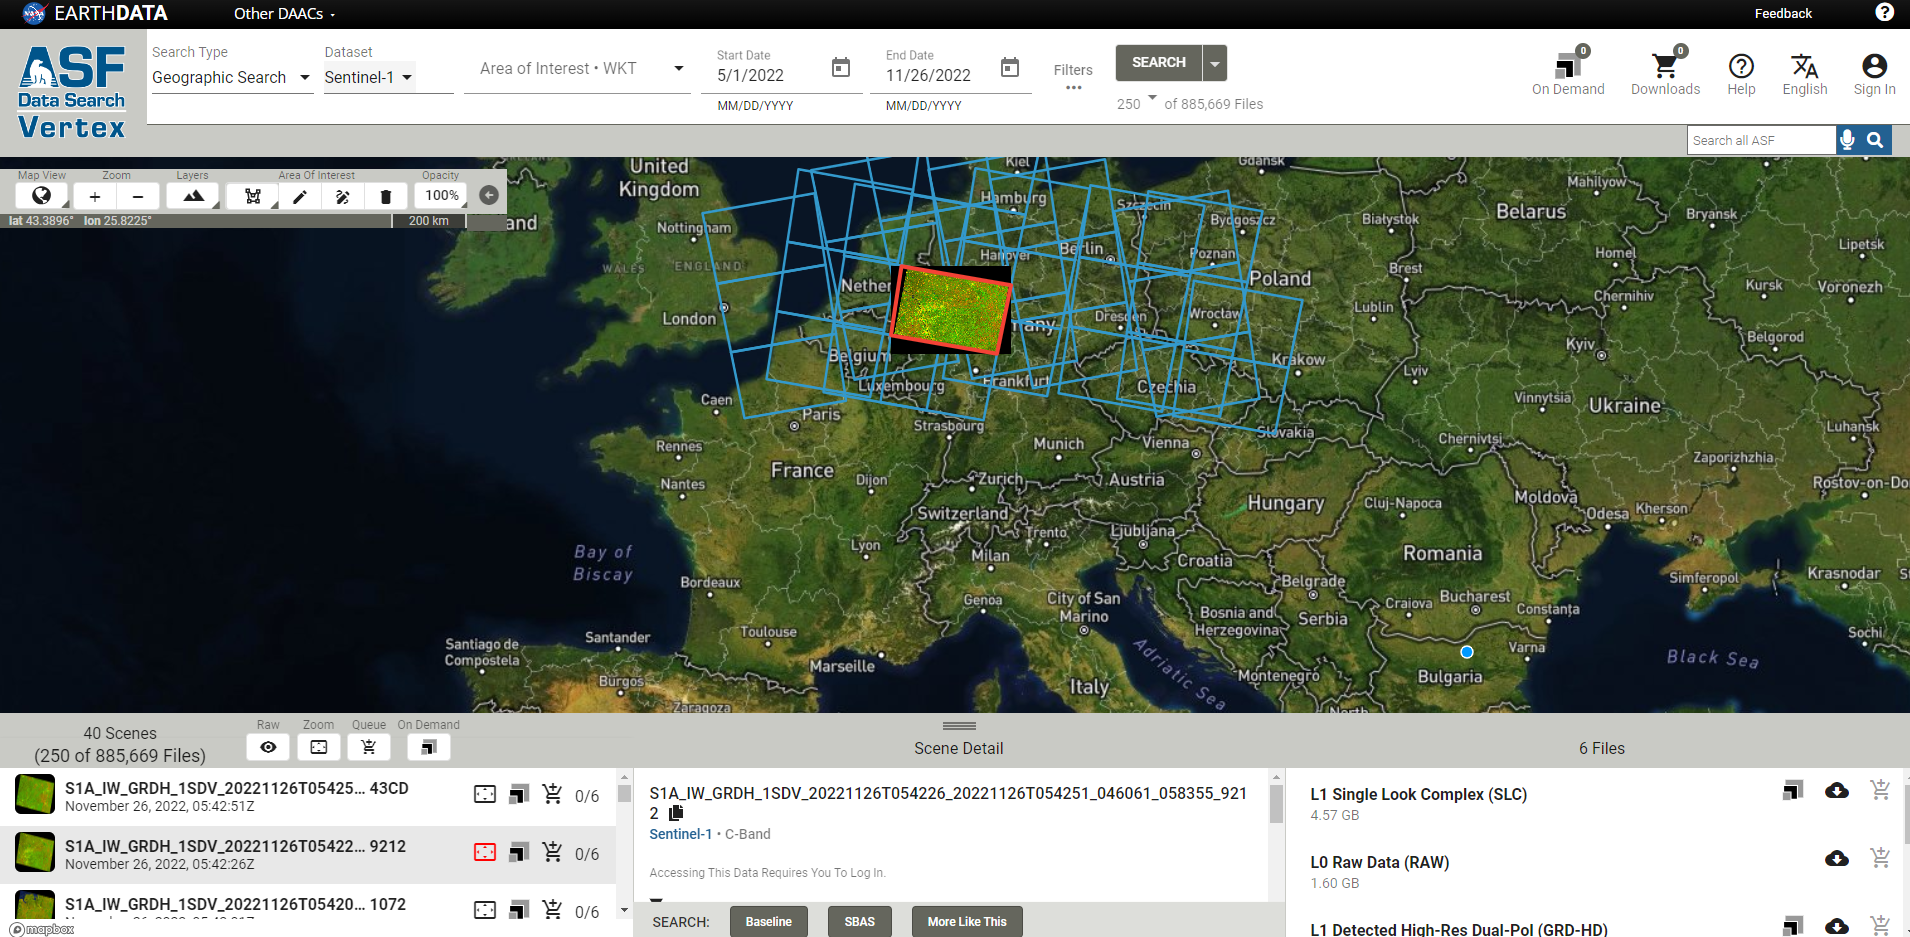
\includegraphics[width=1\textwidth]{../../Images/PNG/alaska1.png}
    %\decoRule
    \caption[Selection of area of interest]{Selection of area of interest.}
    \label{fig:alaska-area1}
\end{figure}

\begin{figure}[H]
    \centering
    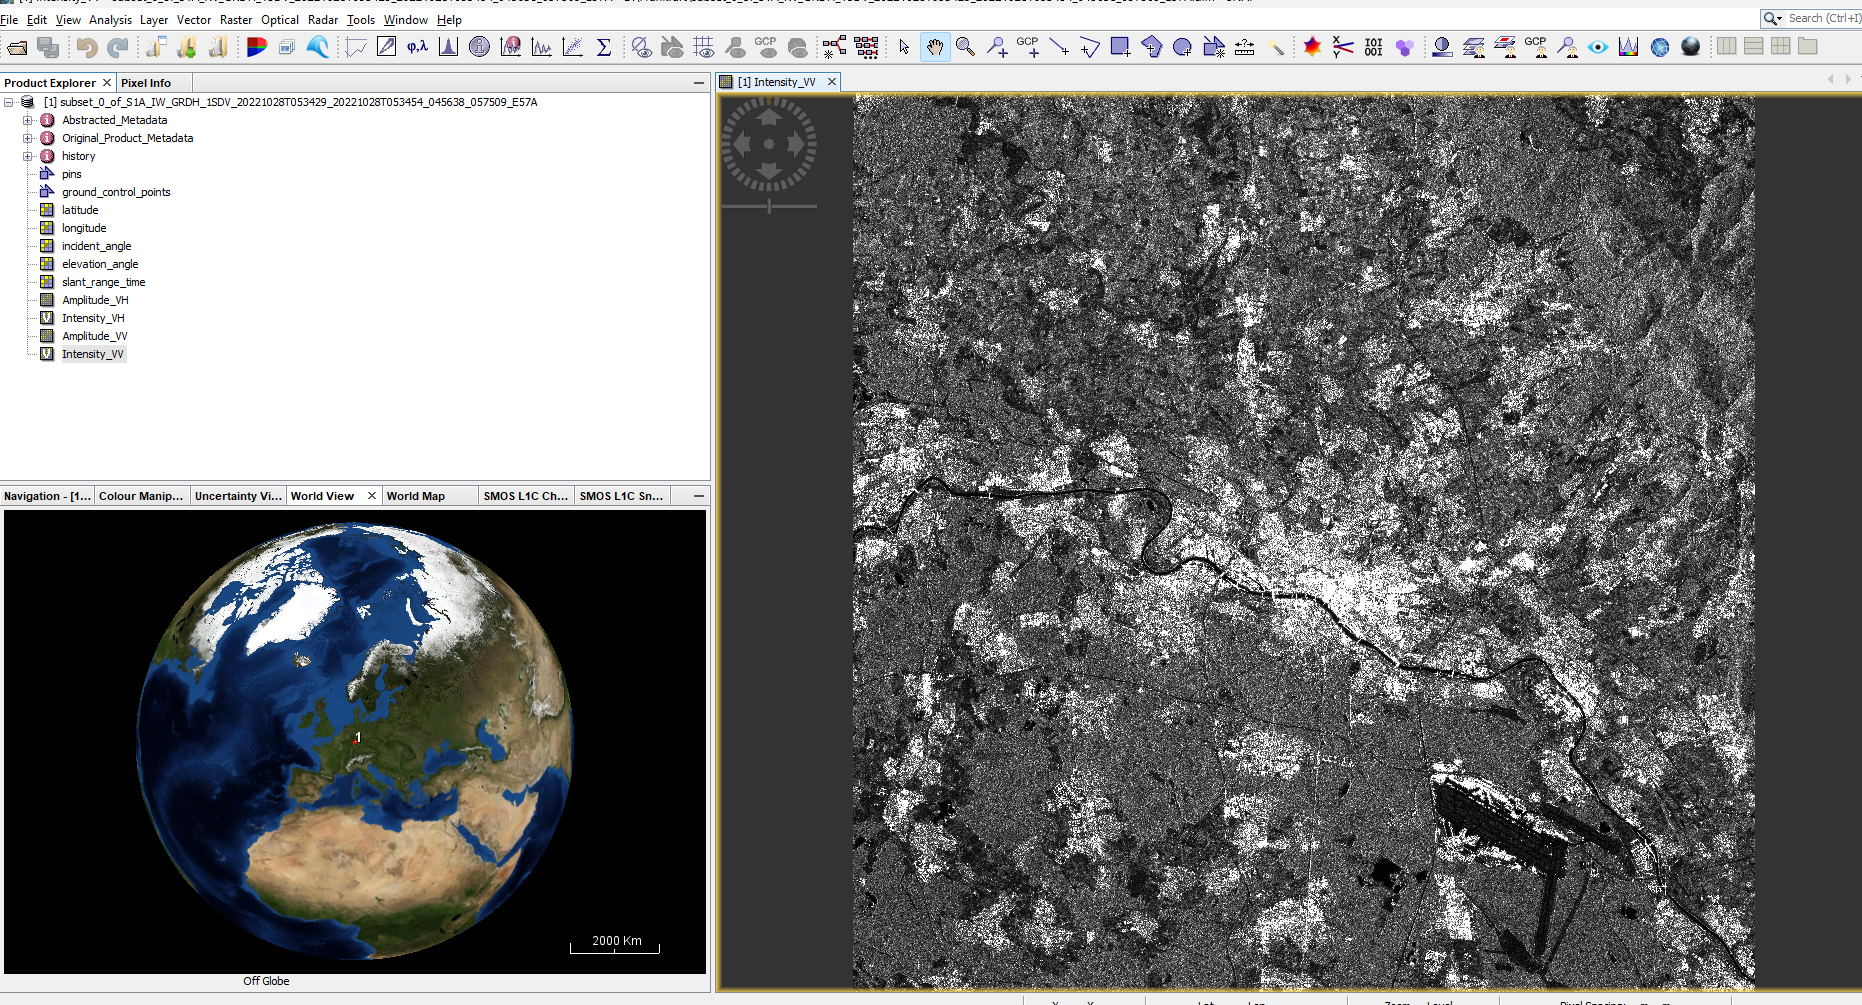
\includegraphics[width=1\textwidth]{../../Images/PNG/snap_1.png}
    %\decoRule
    \caption[SAR Images pre-processing  in the SNAP]{SAR Images pre-processing  in SNAP.}
    \label{fig:alaska-areaf}
\end{figure}






